\documentclass[11pt,a4paper]{article}
\usepackage[utf8]{inputenc}
\usepackage[spanish]{babel}
\usepackage{amsmath}
\usepackage{amsfonts}
\usepackage{amssymb}
\usepackage{graphicx}
\usepackage{float}

\author{Víctor Iranzo}
\title{Capítulo 7: Pruebas}
\setlength{\parskip}{10pt}

\graphicspath{ {Cap7_Images/} }

\begin{document}
\maketitle

\section{Tipos de pruebas}

El siguiente esquema es una modificación del cuadrante de Marick  empleada para catalogar pruebas en distintos tipos:

\begin{figure}[h]
\centering
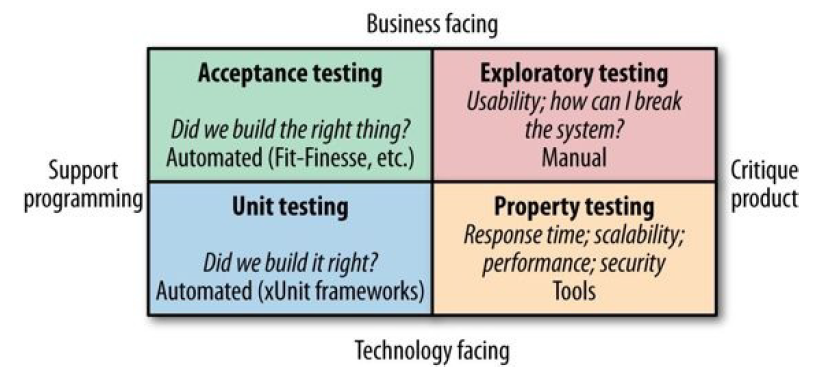
\includegraphics[scale=0.5]{Marick_Quadrant}
\caption{Modificación del cuadrante de Marick hecha por L.Crispin y J.Gregory en su libro Agile Testing.}
\end{figure}

Las pruebas situadas en la mitad inferior están relacionadas con la tecnología empleada, como son las pruebas unitarias o las de rendimiento, que deben ser implementadas por los desarrolladores y que se pueden automatizar. Las pruebas situadas en la mitad superior están orientadas a que los stakeholders conozcan cómo funciona el sistema y que no guardan relación con aspectos tecnológicos. Entran dentro de esta mitad las pruebas de aceptación o las pruebas manuales.

La proporción necesaria de cada tipo de test depende del sistema a desarrollar. La tendencia actual es en favor de los tests de pequeña escala y automatizados. En un sistema basado en microservicios, son esenciales las pruebas de este tipo ya que validarán que no se despliegue a producción código defectuoso.

Podemos clasificar las pruebas en los microservicios en 3 tipos según su alcance: unitarias, de servicios y de extremo a extremo. Estos términos pueden llevar a discusión: por ejemplo, en una prueba unitarias se puede incluir para algunas personas la validación de diferentes clases o funciones mientras que para otras no.

\begin{figure}[h]
\centering
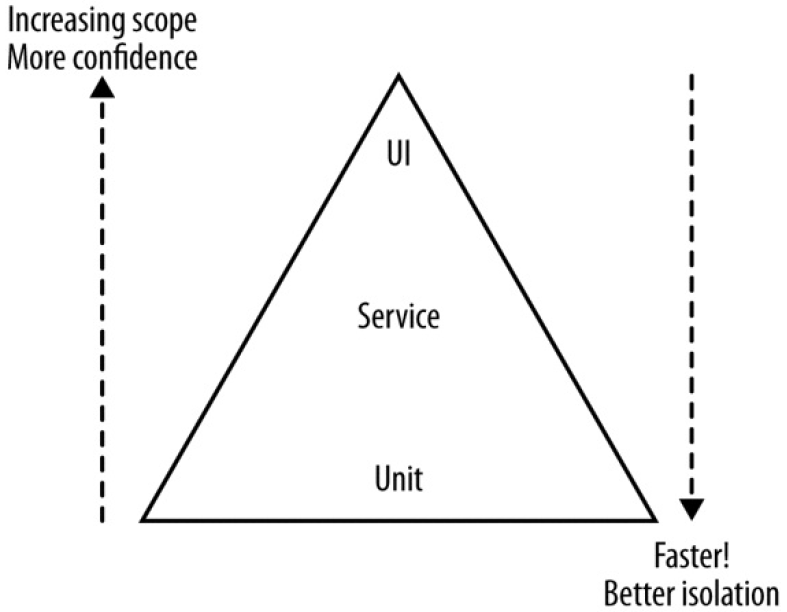
\includegraphics[scale=0.5]{Cohn_Pyramid}
\caption{Pirámide de pruebas diseñada por Mike Cohn en su libro Succeding with Agile.}
\end{figure}


\subsection{Pruebas unitarias}

Son pruebas que validan una única función. Se pueden generar fruto de procesos de desarrollo como el test-driven development (TDD). En general, se prefiere tener un gran número de este tipo de pruebas por su rapidez, porque pueden ayudar a la refactorización del código y porque es donde mayor cantidad de defectos se suele capturar.

\begin{figure}[H]
\centering
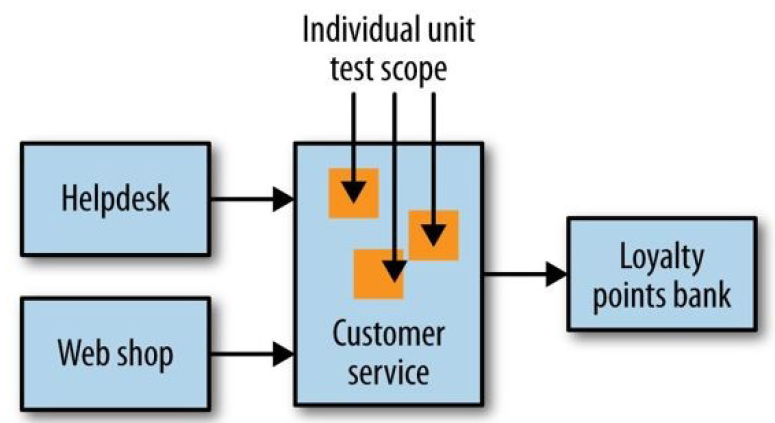
\includegraphics[scale=0.5]{Unit_Tests}
\caption{En las pruebas unitarias no se ejecuta ningún servicio, sino que se prueban métodos específicos de ellos.}
\end{figure}

\subsection{Pruebas de servicios}

En estas pruebas se verifica la funcionalidad de los servicios sin emplear las interfaces de usuario. Cada prueba verifica una de las funcionalidades que el servicio expone. Se pretende comprobar la separación entre los servicios y para solventar las dependencias que el servicio bajo pruebas tiene sobre otros, se reemplazan los servicios colaboradores por stubs o fakes.

Los stubs y los fakes imitan el comportamiento real del servicio al que representan. Los stubs contienen menos lógica que los fakes y ante una petición responden siempre de la misma manera. Por su parte, los fakes pueden emplearse para comprobar que los efectos secundarios de la interacción entre los servicios ocurre. Por ejemplo, si al invocar a un servicio el comportamiento esperado es que este añada una tupla en base de datos, un stub podría responder simplemente con un 200 OK mientras que un fake tendría más lógica para reproducir esto.

Este tipo de pruebas pueden ser igual de rápidas que las unitarias siempre que no se tengan que emplear un gran número de infraestructuras como bases de datos o redes.

\begin{figure}[h]
\centering
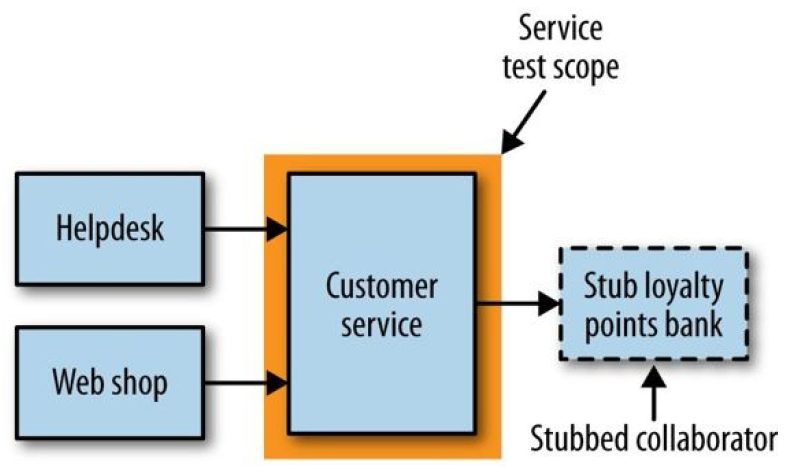
\includegraphics[scale=0.5]{Service_Tests}
\caption{Las pruebas de servicio se ejecutan sobre un único servicio y emplean fakes para reemplazar a los colaboradores de este.}
\end{figure}

\subsection{Pruebas de extremo a extremo}

Son pruebas que se ejecutan sobre todo el sistema. Cubren gran parte de código, por lo que su correcta ejecución dan mucho grado de confianza. En su ejecución se levantan varios servicios diferentes.

De los servicios que se prueban, ¿qué versión se debe emplear de cada uno? ¿Quién debe poder ejecutar esta prueba? Cada vez que se realice un cambio en alguno de los participantes deberían ejecutarse todas las pruebas en las que este se emplea. Una manera elegante de conseguir esto es hacer que en la compilación de la integración continua, la fase de pruebas de extremo a extremo sea compartida entre todos los involucrados para que las pruebas se ejecuten cada vez que cambie uno de ellos y la versión a probar de todos sea la asociada al cambio.

\begin{figure}[h]
\centering
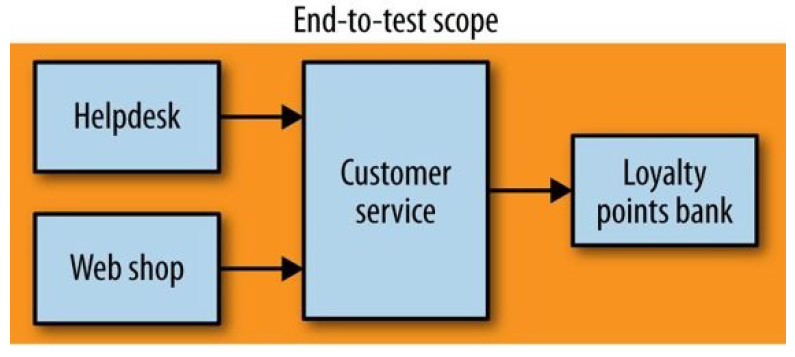
\includegraphics[scale=0.5]{End_To_End_Test}
\caption{Las pruebas de servicio se ejecutan sobre un único servicio y emplean fakes para reemplazar a los colaboradores de este.}
\end{figure}

\subsubsection{Desventajas de las pruebas de extremo a extremo}

\begin{itemize}

\item Pruebas frágiles: conforme el alcance del test aumenta mayor son las partes bajo prueba sobre las que no se puede tener control. Estas partes pueden introducir fallos que no demuestran que la funcionalidad tenga un defecto, sino fallan porque otro problema ha ocurrido como puede ser un fallo en la red. Las pruebas así son menos deterministas y el desarrollador puede acostumbrarse a que fallen si consigue hacerlas pasar al ejecutarlas por segunda vez, lo que se conoce como normalizar la desviación. Este tipo de pruebas han de ser eliminadas cuanto antes de la suite de pruebas y refactorizadas en pruebas de menor alcance.

\item Responsable de las pruebas: si los servicios que participan en las pruebas son mantenidos por distintos equipos, es necesario que todos ellos se hagan responsables de la suite de pruebas. Diferentes situaciones pueden ocurrir sino:

\begin{itemize}

\item Explosión de pruebas: si nadie controla la salud de la suite, los equipos pueden añadir pruebas descontroladamente que no aporten valor.

\item Ignorar resultados de las pruebas: cuando una prueba falla, nadie trata de arreglarla porque cree que la responsabilidad la tiene otro.

\item Equipos especializados en pruebas: esto puede alargar el tiempo de desarrollo de una funcionalidad por requerir mayor coordinación entre equipos. Además, con esta metodología los desarrolladores se involucran menos en las pruebas, haciendo su código más difícil de probar e ignorando los resultados de las pruebas.

\end{itemize}

\item Tiempo de ejecución mayor: al levantar un mayor número de servicios y cubrir más código se alarga el tiempo de ejecución de la prueba. Esto puede ser sobrellevado a través de la ejecución en paralelo de pruebas. Esto combinado con la fragilidad de los tests puede desencadenar que encontrar la causa del fallo de una prueba requiera de un mayor esfuerzo.

\item Mayor tiempo de retroalimentación: si las pruebas tardan más en ejecutarse, el desarrollador tardará más tiempo en darse cuenta de que en los cambios realizados ha introducido un defecto. Este hecho puede repercutir en el resto del equipo, ya que si la compilación está rota debido a una prueba que no pasa, los cambios que otros suben pueden apilarse, dificultando su futura integración.

\end{itemize}

\section{Balance de pruebas a realizar}

Si volvemos a la pirámide de Cohn, uno de los conceptos clave es que a medida que aumenta el alcance las pruebas lo hace el nivel de confianza que las pruebas dan sobre la ausencia de defectos. Por otro lado, cuanto más arriba en la pirámide más tiempo tardará una prueba en ejecutarse y dar retroalimentación al desarrollador. Además, determinar el motivo de fallo de una prueba será más costoso cuanto mayor sean las líneas de código probadas.

El número de pruebas que se aconseja tener de cada tipo aumenta conforme descendemos por la pirámide. Un antipatrón sería seguir como convención la misma pirámide invertida. En este caso, nuestra cobertura de pruebas se basaría en pruebas de largo alcance y larga ejecución, nada deseable según los principios de integración continua.

En cuanto a las pruebas de extremo a extremo, no podemos añadir una prueba de este tipo por cada nueva funcionalidad que el sistema ofrezca. El número de servicios que participan para ofrecer una funcionalidad puede ser muy alto y en una prueba no se deberían de levantar más de 3 o 4 servicios para no potenciar las desventajas que hemos mencionado.

\section{Pruebas frágiles y escamosas}

\section{Pruebas antes de producción}

\subsection{Despliegues verde y azul}

\subsection{Canary releases}

\subsection{Tiempo medio entre fallos y tiempo medio entre reparaciones}

\section{Pruebas de requisitos no funcionales}

\subsection{Pruebas de rendimiento}

\end{document}